\section{学習過程}
本章では,Unity ML-Agentsを用いた車エージェントの学習プロセスについて詳しく記述する.
\subsection{基本操作の学習}
エージェントは,初期段階で車の基本的な操縦技術を身につける.これには,加速,減速,方向転換といった基本的な車両操作の理解と,これらの操作を組み合わせて車両をコントロールする訓練が含まれる.報酬システムを通じて,エージェントは道路を無事に一周することで基本的な車両制御スキルを獲得する.基本操作の学習の様子を図13に示す.
\begin{figure}[H]
    \centering
    \includegraphics[width=0.8\textwidth]{figures/BasicMovement1.eps} % ここで図のファイル名とサイズを指定します
    \caption{基本操作の学習} % 図のキャプション
    \label{fig:basic-movement-2} % 図への参照用ラベル
\end{figure}

\subsection{静止している障害物}
基本操作の学習後,エージェントは静止している障害物を回避する技術を学習する.この段階では,ランダムに配置された2つの障害物を検出し,それを安全に回避しながら道路を進む戦略を身に着けることが求められる.学習成果として,エージェントは静的な障害物を効果的に避ける能力を示す.車エージェントが静止している障害物を避ける様子を以下の図14に示す.
\begin{figure}[H]
    \centering
    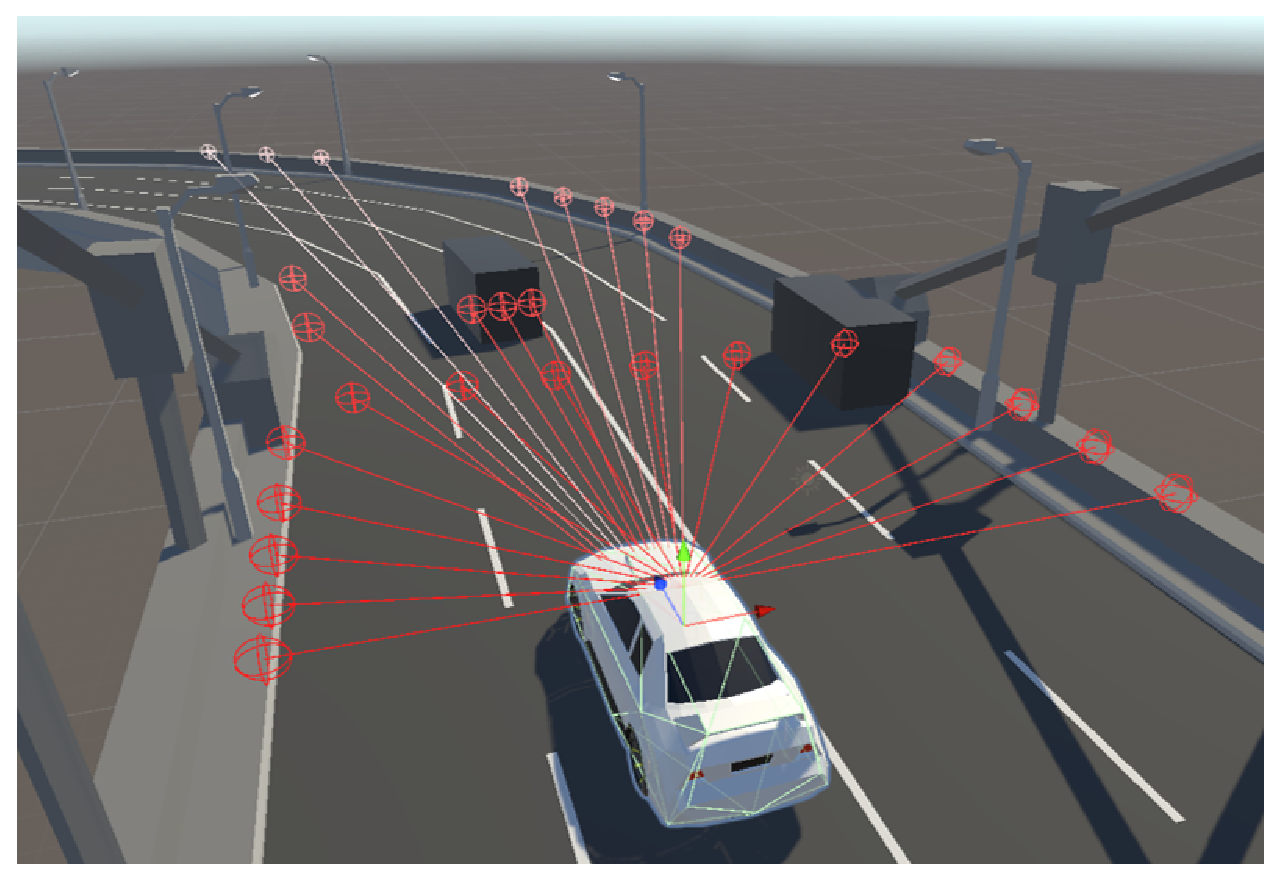
\includegraphics[width=0.8\textwidth]{figures/NonMovingObstacle.eps} % ここで図のファイル名とサイズを指定します
    \caption{静止している障害物} % 図のキャプション
    \label{fig:non-moving-obstacle} % 図への参照用ラベル
\end{figure}

\subsection{障害物の速度上昇}
さらに学習を進んで,エージェントは動的障害物,特にその速度を上げた障害物に対応することを学習する.障害物の数は2個から11個まで増やし,これによりエージェントはより複雑な環境下で運転する技術を習得する.より速い速度の障害物を回避するために,エージェントは予測と即時反応の両方が向上する.数が増えた障害物の学習を以下の図15に示す.
\begin{figure}[H]
    \centering
    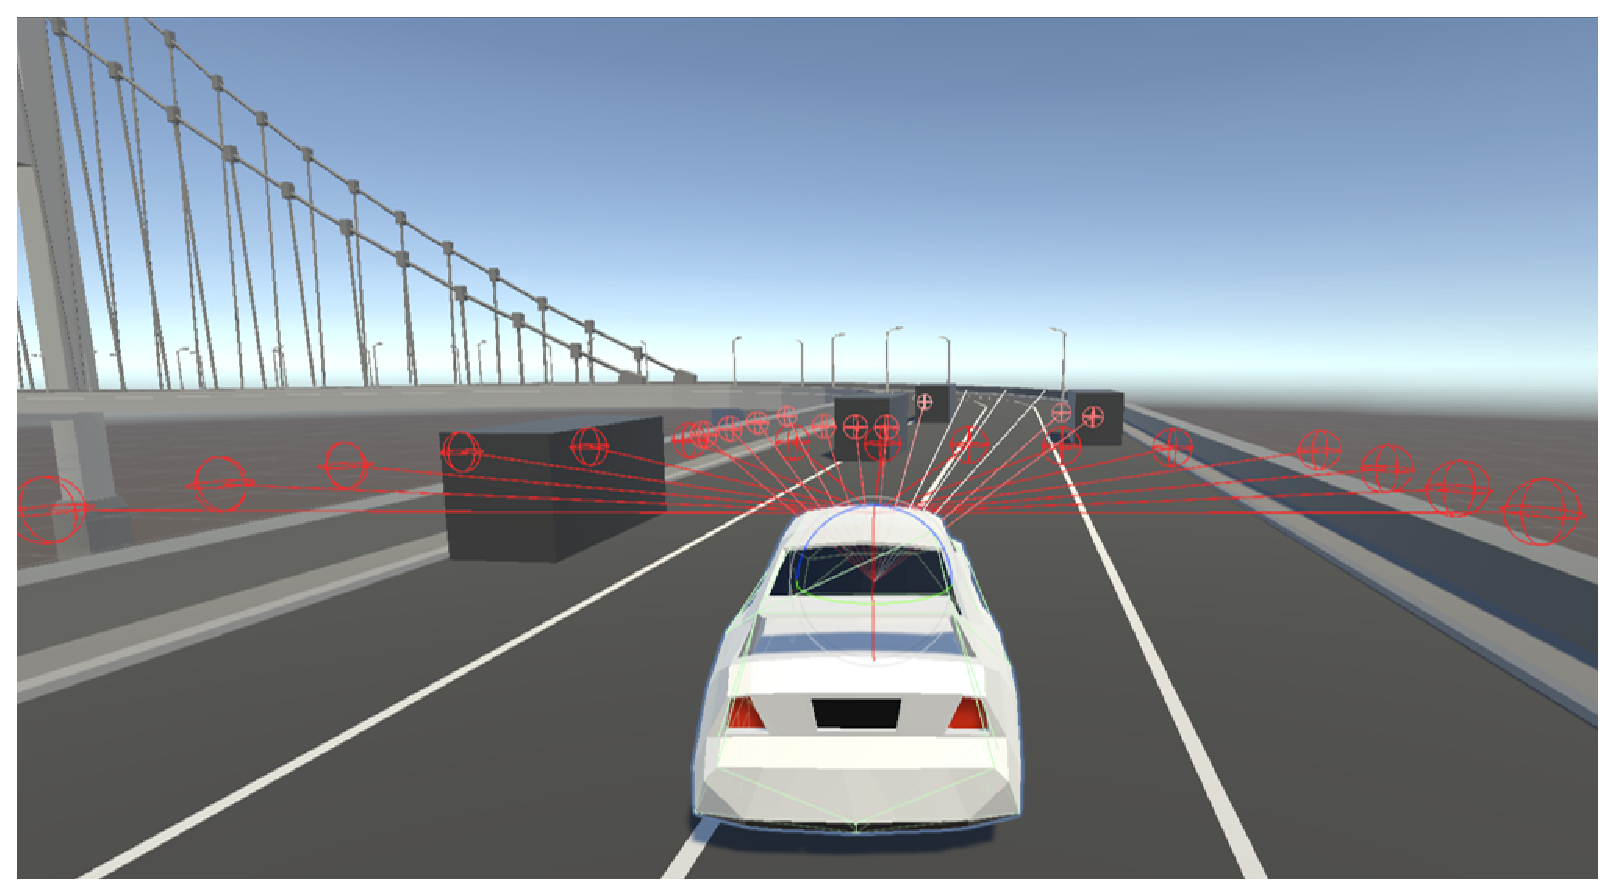
\includegraphics[width=0.8\textwidth]{figures/MovingObstacles.eps} % ここで図のファイル名とサイズを指定します
    \caption{障害物の速度上げと増えた数} % 図のキャプション
    \label{fig:moving-obstacles} % 図への参照用ラベル
\end{figure}

\subsection{四車線一方通行}
学習プロセスは次に,四車線一方通行のシナリオへと移る.この環境では,エージェントは追い越しを行うスキルを学習した.この段階での学習により,エージェントは一方通行の環境における複数車両の動きに適応する能力を示す.四車線一方通行の学習様子を以下の図16に示す.
\begin{figure}[H]
    \centering
    \includegraphics[width=0.8\textwidth]{figures/OneWayTraffic.eps} % ここで図のファイル名とサイズを指定します
    \caption{四車線一方通行} % 図のキャプション
    \label{fig:one-way-traffic} % 図への参照用ラベル
\end{figure}

\subsection{四車線対面通行}
最終的に,エージェントは四車線対面通行という,より高度な運転環境での学習を行う.対面通行のシナリオでは,エージェントは対向車線から来る車両と衝突を避けるための判断能力を高める必要があった.この環境での学習結果を一方通行の結果と比較することで,エージェントの適応能力と戦略の違いを明確になる.四車線対面通行の学習様子を以下の図17に示す.
\begin{figure}[H]
    \centering
    \includegraphics[width=0.8\textwidth]{figures/TwoWayTraffic.eps} % ここで図のファイル名とサイズを指定します
    \caption{四車線対面通行} % 図のキャプション
    \label{fig:two-way-traffic} % 図への参照用ラベル
\end{figure}

全体的に,本章はエージェントの学習プロセスを段階的に丁寧に説明している.各段階でのエージェントの目標とそれを達成するための方法,およびその結果が記述されている.報酬システムがエージェントの行動選択をどのように促し,学習を導いているかも効果的に示されている.

\subsection{学習結果}
\subsubsection{四車線一方通行の学習結果}
\begin{table}[H]
\centering
\caption{四車線一方通行の学習結果}
\label{tab:ippoutuukou}
\begin{tabular}{|c|c|c|c|c|}
\hline
\multirow{2}{*}{走行時間} & \multicolumn{4}{c|}{対向車なし} \\ \cline{2-5} 
                           & 50s & 100s & 150s & 200s \\ \hline
No. 1                       & 0   & 2    & 3    & 4    \\ \hline
No. 2                       & 0   & 1    & 3    & 2    \\ \hline
No. 3                       & 0   & 2    & 0    & 1    \\ \hline
No. 4                       & 1   & 0    & 3    & 3    \\ \hline
No. 5                       & 0   & 1    & 2    & 3    \\ \hline
No. 6                       & 0   & 0    & 2    & 5    \\ \hline
No. 7                       & 0   & 1    & 1    & 3    \\ \hline
No. 8                       & 0   & 2    & 2    & 2    \\ \hline
No. 9                       & 0   & 1    & 3    & 1    \\ \hline
No.10                      & 0   & 1    & 2    & 3    \\ \hline
平均                       & 0.1 & 1.1  & 2.1  & 2.7  \\ \hline
最高値                     & 1   & 2    & 3    & 5    \\ \hline
最低値                     & 0   & 0    & 0    & 1    \\ \hline
\end{tabular}
\end{table}
四車線一方通行のシナリオでの学習結果を示す表1は,各エピソードの走行時間(50秒,100秒,150秒,200秒)で10回実施したテストの結果である.グラフから分かるように,エピソードの時間が増えるにつれて平均衝突回数がわずかに増加する傾向が見られる.具体的には,50秒の走行では平均衝突回数が0.1回,200秒の走行では平均2.7回となっている.この結果から,走行時間が長くなるほど,車エージェントが直面するシナリオの数が増え,それに伴い衝突の可能性も高まることが示される.

このシナリオでは,最低値と最高値のデータを見ると,あるテストでは全く衝突が発生しないもあれば,最大で5回の衝突が発生する場合もあり,エージェントのパフォーマンスには個別の差があることが分かる.

\subsubsection{四車線対面通行の学習結果}
四車線対面通行についての学習結果を以下の表2に示す.
\begin{table}[H]
\centering
\caption{四車線対面通行の学習結果}
\label{tab:taimentuukou}
\begin{tabular}{|c|c|c|c|c|}
\hline
\multirow{2}{*}{走行時間} & \multicolumn{4}{c|}{対向車あり} \\ \cline{2-5} 
                           & 50s & 100s & 150s & 200s \\ \hline
No. 1                       & 0   & 2    & 3    & 6    \\ \hline
No. 2                       & 0   & 4    & 4    & 3    \\ \hline
No. 3                       & 0   & 1    & 3    & 3    \\ \hline
No. 4                       & 1   & 1    & 2    & 4    \\ \hline
No. 5                       & 0   & 2    & 4    & 6    \\ \hline
No. 6                       & 0   & 2    & 4    & 2    \\ \hline
No. 7                       & 0   & 1    & 1    & 2    \\ \hline
No. 8                       & 1   & 2    & 5    & 3    \\ \hline
No. 9                       & 0   & 1    & 3    & 3    \\ \hline
No.10                      & 1   & 2    & 4    & 4    \\ \hline
平均                       & 0.3 & 1.8  & 3.3  & 3.6  \\ \hline
最高値                     & 1   & 4    & 5    & 6    \\ \hline
最低値                     & 0   & 1    & 1    & 2    \\ \hline
\end{tabular}
\end{table}
表2を見ると,四車線対面通行のシナリオでは,一方通行のシナリオと比較して,全体的に平均衝突回数が高くなっている.特に200秒の走行では平均衝突回数が3.6回に達しており,これは対面通行が一方通行よりもエージェントにとって運転が難しい状況であることを示している.エージェントは自車線の障害物だけでなく,対向車線から接近する障害物にも対応する必要がり,対向車の有無のシナリオにより予測すべき変数が変化するため,より良い運転方法を学習することが難しくなることに起因すると考えられる.

\subsection{考察}
最終的な学習結果から,四車線一方通行のシナリオではエージェントが比較的良い成果を示した一方で,対面通行のシナリオにおいてはまだ改善の余地があると考えられる.\\







